\documentclass{scrbook}

% Language setting
% Replace `english' with e.g. `spanish' to change the document language
\usepackage[english]{babel}

% Set page size and margins
% Replace `letterpaper' with `a4paper' for UK/EU standard size
\usepackage[a4paper,top=2cm,bottom=2cm,left=3cm,right=3cm,marginparwidth=1.75cm]{geometry}

\setkomafont{author}{\scshape}
\usepackage{blindtext}

% Useful packages
\usepackage{amsmath}
\usepackage{graphicx}
\usepackage[colorlinks=true, allcolors=blue]{hyperref}

\usepackage{layouts}

\usepackage{caption}
\usepackage{subcaption}

\title{Optimal Vehicle Maneuvers}
\author{Arvind Balachandran\thanks{I sometimes procrastinate}}
\subtitle{Not a course in vehicle dynamics, of course!}
\subject{Technical Report}

\usepackage{xspace}
\newcommand{\uvec}[1]{\textit{$\textit{u}_{\textit{#1}}$}\xspace}
\newcommand{\tsim}{\textit{$\textit{t}$}\xspace}
\newcommand{\mass}{\textit{$\textit{m}$}\xspace}

\usepackage{matlab-prettifier}

\usepackage{tikz}

\begin{document}
\maketitle

\chapter[Particle model optimization]{Friction-limited particle with and without rate-limitation}
Investigating the friction-limited particle and the friction-limited particle with rate-limited direction control with a comparison. 

The optimization problems follow the following general equation structure: 
\begin{align}
    & \underset{u}{\text{Min}}
    & & J\\
%
    & \text{subject to} 
    & & f_u(u) <= 0\\
%
    &&& f_o(x,u) <= 0 \\
%
    &&& \dot x = f(x,u),\\
%
    &&& x_0,\ x_f,
\end{align}
where $u$ is(are) the optimization variable(s), $J$ is the cost function, $f_u(u) <= 0$ and $f_o(x,u) <= 0$ denote the constraints on the $u$ and the states $x$, $\dot x = f(x,u)$ are the ODEs or dynamic constraints, and $x_0,\ \&\ x_f$ are the boundry conditions. 

\begin{description}
    \item[Opimization variables:] the longitudinal and lateral forces $u_x$ and $u_y$ on the vehicle. 
    \item[Cost function:] to minimize time $t$.
    \item[Constraints:] The forces on the vehicle are limited elliptically, i.e., \begin{equation*}
        u_x^2 + u_y^2 \leq (\mu m g)^2.
    \end{equation*}
    The force limit on the vehicle for the rate-limited direction control is given by \begin{align*}
        u_1^2 \leq (\mu m g)^2.
    \end{align*}\par The obstacle is given by the following equation:
    \begin{align*}
        \left(\frac{x - X_a}{R_1}\right)^n + \left(\frac{y}{R_2}\right)^n \geq 1
    \end{align*}
    \item[Vehicle model:] The friction-limited particle is given as follows: \begin{align*}
        \dot x &= v_x, \\
        \dot x &= v_x, \\
        m\,\dot v_x &= u_x,\\
        m\,\dot v_x &= u_y. \\
    \end{align*}
    The friction-limited particle with rate-limited direction control is given as follows: \begin{align*}
        \dot x &= v_x, \\
        \dot x &= v_x, \\
        m\,\dot v_x &= u_1\,\cos\left(\delta\right),\\
        m\,\dot v_y &= u_1\,\sin\left(\delta\right), \\
        \dot \delta &= u_2. \\
    \end{align*}
    \item[Miscellaneous constraints:] In order to ensure that the solution is within the desired operating space, certain miscellaneous constraints are included such as, \begin{align*}
        x_0 \leq x \leq x_f\\
        y_0 \leq y \leq y_f\\
        y_{min} \leq y \leq y_{max} \\
        0 \leq v_x 
    \end{align*} 
    For the rate-limited direction control model, the steering angle and steering rate is also constrained, i.e., \begin{align*}
        |\delta| \leq \delta_{max}, \\
        |\dot\delta| \leq \dot\delta_{max}, \\
    \end{align*}
\end{description}

The model, optimization, and obstacle parameters are presented in Tables~\ref{tab:flp_mdlparams},~\ref{sub@tab:flp_optparams}, and~\ref{sub@tab:flp_obsparams}, respectively. 

\begin{table}[h!]
    \begin{subtable}[h]{0.3\textwidth}
        \centering
        \begin{tabular}{c|c}
            - & value \\
            \hline
            $m$ & 500\,kg\\
            $g$ & 9.8\,m/s\textsuperscript{2}\\
            $\mu$ & 0.8\\
        \end{tabular}
        \caption{Model parameters}
        \label{tab:flp_mdlparams}
    \end{subtable}
    \hfill
    \begin{subtable}[h]{0.3\textwidth}
        \centering
        \begin{tabular}{c|c}
            - & value \\
            \hline
            $x_0$ & 0\,m\\
            $x_f$ & 100\,m\\
            $y_0$ \& $y_f$ & 1\,m\\
            $v_x$ & 40\,km/h\\
            $v_y$ & 0\,km/h
        \end{tabular}
        \caption{Initial parameters}
        \label{tab:flp_optparams}
    \end{subtable}
    \hfill
    \begin{subtable}[h]{0.3\textwidth}
        \centering
        \begin{tabular}{c|c}
            - & value \\
            \hline
            $X_a$ & 50\,m\\
            $R_1$ & 2\,m\\
            $R_2$ & 1.5\,m\\
            $n$ & 6\\
        \end{tabular}
        \caption{Obstacle parameters}
        \label{tab:flp_obsparams}
    \end{subtable}
    \caption{Model, optimization, and obstacle parameters.}
    \label{tab:temps}
\end{table}

The optimal control problem (OCP), was solved with direct multiple-shooting with 40 control intervals for the optimization using Matlab and CasADi. The ODE was solved using the fixed-step Runge-Kutta 4 integration method. 

The results of the optimization are presented in 

\begin{figure}[h!]
    \centering
    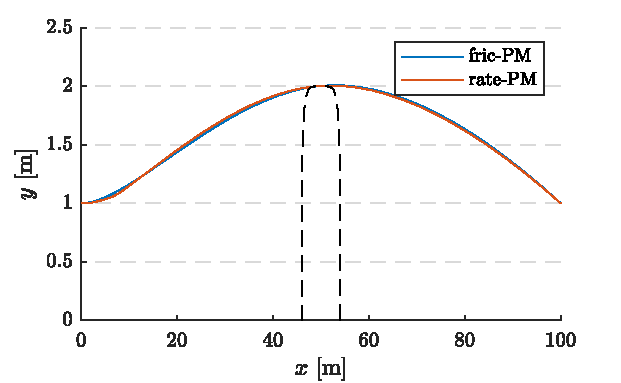
\includegraphics{figures/flp_avoid.pdf}
    \caption{Obstacle avoidance trajectory for the friction- and rate-limited particle model.}
    \label{fig:res_traj_p1}
\end{figure}

\pagebreak

\begin{table}[h]
    \centering
    \begin{tabular}{c|c|c}
        - & min $t$ & min $-v_f$ \\
        \hline
        $t$ & 3.83\,s & 3.94\,s \\
        $v_x(t_f)$ & 147.59\,km/h & 146.03\,km/h\\
    \end{tabular}
    \caption{Results for friction-limited and rate-limited particle model.}
    \label{tab:prob1_res}
\end{table}

From Table~\ref{tab:prob1_res}, it is clear that the friction-limited particle model (fric-PM) is slightly faster than the rate-limited particle model (rate-PM). 
This is because in rate-PM the rate of change of direction of the particle is limited and as a result, the ability of the vehicle to make a sharp turn is restricted and thus takes a longer time to complete the maneuver. 
This is visible in the control signals and state variables for the optimal trajectory shown in Figure~\ref{fig:prob1_res_detail}. 

Additional constraints and initial values for the firc-PM and rate-PM are presented in Table~\ref{tab:const_p1}. 

\begin{table}[h]
    \centering
    \begin{subtable}[h]{0.4\textwidth}
        \begin{tabular}{c|c||c|c}
            \multicolumn{2}{c||}{fric-PM} & \multicolumn{2}{c}{rate-PM}\\
            \hline
            $y_{max}$ & 5 & $\delta_{max}$ & $\pi/2$ \\
            - & - & $\dot\delta_{max}$ & $\pi/6$ 
        \end{tabular}
        \caption{Constraints.}
        \label{tab:const_p1a}
    \end{subtable}
    % \hfill
    \begin{subtable}[h]{0.4\textwidth}
        \begin{tabular}{c|c||c|c}
            \multicolumn{2}{c||}{fric-PM} & \multicolumn{2}{c}{rate-PM}\\
            \hline
            $v_x$ & 40\,km/h & $v_x$ & 40\,km/h
        \end{tabular}
        \caption{Initial conditions.}
        \label{tab:const_p1a}
    \end{subtable}
    \caption{Constraints for the fric-PM and rate-PM.}
    \label{tab:const_p1}
\end{table}

\begin{figure}[h!]
    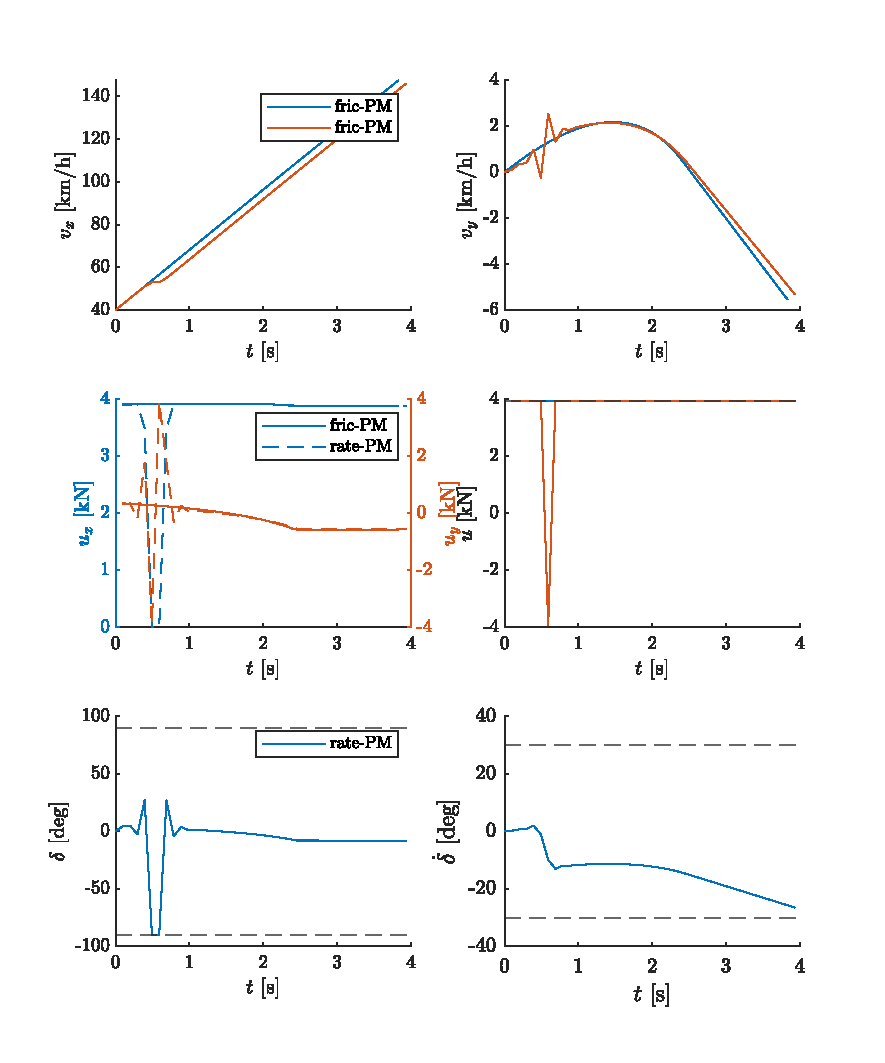
\includegraphics{figures/flp_avoid_detailed.pdf}
    \caption{Detailed optimal trajectory states and control inputs for friction- and rate-limited particle models.}
    \label{fig:prob1_res_detail}
\end{figure}

\noindent\fbox{%
    \parbox{\textwidth}{%
        \textbf{Some reflections}: \newline
        The fric-PM can converge faster than the rate-PM in some cases. 
        Since 'ipopt' is used to solve the optimization problem, fric-PM is more sensitive toward the initializations (initial guesses). 
        Therefore, additional constraints may be necessary to improve convergence.
        Furthermore, the rate-PM does not have this problem and thus can have a lower computational time.
        However, the computational time can get long with 'bad' initialization conditions. 
        The convergence of this model seems better than the fric-PM.
        
        It is worth mentioning that the terms 'improved convergence' and 'better convergence' mean the ability of the solver to produce an 'optimal solution found' even with ridiculous guesses. However, one should take care not to fall into local minima pits. 
    }%
}

\section{Code}
The source code for this problem can be found at \newline \href{https://github.com/arvba41/optimal_vehicle_maneuvers/tree/main/uppgift/ugf1}{https://github.com/arvba41/optimal\_vehicle\_maneuvers}.
\chapter[Double-Track Maneuver Optimization]{Maneuver with DT for hairpin 4\textsuperscript{th} degree super ellipse, without LT or WT.}

In addition to the double-track (DT) model equations state equations,
% \begin{align*}
%     \dot X_p &= v_x\,\cos(\psi) - v_y\,\sin(\psi),\\
%     \dot Y_p &= v_x\,\sin(\psi) + v_y\,\cos(\psi),\\
%     \dot \psi &= r,\\
%     \dot v_x &= \frac{F_x}{m} + v_y\,r,\\
%     \dot v_Y &= \frac{F_Y}{m} + v_x\,r,\\
%     \dot r &= \frac{M_z}{I_{zz}}.
% \end{align*}
the input forces are filtered using a low pass filter with a time constant $\tau_f$ to prevent NaN errors during the optimization.
\begin{align}
    \dot F_{x(f)} &= \frac{1}{\tau_f}\,\left(F_{x(f)}^* - F_{x(f)}\right),\\
    \dot F_{x(r)} &= \frac{1}{\tau_f}\,\left(F_{x(r)}^* - F_{x(r)}\right),
\end{align}
where $F_{x(f)}^*$ and $F_{x(r)}^*$ are the inputs to the model.

The hairpin is modeled as two ellipses,
\begin{align}
    \frac{x}{R_1^i} + \frac{y}{R_2^i} & \geq 1, & \frac{x}{R_1^o} + \frac{y}{R_2^o} & \leq 1.
    % \frac{x}{R_1^î} + \frac{y}{R_2^i} &\geq 1 \ \text{Inner ellipse},
    % \frac{x}{R_1^o} + \frac{y}{R_2^o} &\leq 1 \ \text{outer ellipse}.
\end{align}
A straightforward model of combined forces is based on the friction ellipses and the Magic Formula. The tire parameters are taken from Berntorp, Karl, et al. "Models and methodology for optimal trajectory generation in safety-critical road–vehicle manoeuvres." Vehicle System Dynamics 52.10 (2014): 1304-1332.

The nominal normal force $F_z$ resting on the respective wheel in the steady state is given by
\begin{align}
    F_{z(1)} &= \frac{1}{2}\,mg\frac{l_r}{l_f+l_r}, & F_{z(2)} &= \frac{1}{2}\,mg\frac{l_r}{l_f+l_r}, & F_{z(3)} &= \frac{1}{2}\,mg\frac{l_f}{l_f+l_r}, & F_{z(4)} &= \frac{1}{2}\,mg\frac{l_f}{l_f+l_r}.
\end{align}

\section{Constrains}
\begin{description}
    \item[$v_x > 0$] to avoid $\div$ by zero error while calculating the lateral slips, $\alpha$.
    \item[$-\delta_{max} \leq \delta \leq \delta_{max}$] steering angle limit.
    \item[$-\dot\delta_{max} \leq \dot\delta \leq \dot\delta_{max}$] steering angle rate limit.
    \item[$-\epsilon\,D_{x(f)} \leq F_{x(f)}^* \leq \epsilon\,D_{x(f)}$], limiting the forces on the front wheel, and $\epsilon$ is a number close to 1 to avoid NaN errors. 
    \item[$-\epsilon\,D_{x(r)} \leq F_{x(r)}^* \leq 0$], limiting the forces on the rear wheel.
    \item[$X_f - \beta \leq X_p(\text{end}) \leq X_f + \beta $], Allowing some error on the final $X_P$.
    \item[$Y_f - \beta \leq Y_p(\text{end}) \leq Y_f + \beta $], Allowing some error on the final $Y_P$.
\end{description}
The model is front-wheel driven but can brake on all four wheels.

\section{Cost function}
The const function $J$ is defined as 
\begin{align}
    J &= \min{\left(t + 0.5\beta\right)},
\end{align}
The number 0.5 is arbitrarily chosen. 

The vehicle parameters and constraints for the the optimal control problem are presented in Table \ref{tab:ocp_prob2}.

\begin{table}[h!]
    \begin{subtable}{0.3\textwidth}
        \begin{tabular}{c|c}
            parameter & value\\
            \hline
            $m$ & 2100\,kg\\
            $l_f$ & 1.3\,m \\     
            $l_r$ & s1.5\,m \\
            $w$ & 0.8\,m\\
            $g$ & 9.82\,m/s\textsuperscript{2}\\
            $I_{zz}$ & 3900\,kgm\textsuperscript{2}\\
        \end{tabular}
        \caption{Vehicle parameters}
    \end{subtable}
    \hfill
    \begin{subtable}{0.3\textwidth}
        \begin{tabular}{c|c}
            parameter & value\\
            \hline
            $R_1^i$ & 2\,m \\
            $R_2^i$ & 50\,m \\
            $R_1^o$ & 7\,m \\
            $R_2^o$ & 55\,m \\
        \end{tabular}
        \caption{Hairpin parameters}
    \end{subtable}
    \hfill
    \begin{subtable}{0.3\textwidth}
        \begin{tabular}{c|c}
            parameter & value\\
            \hline
            $\delta_{max}$ & 30$^\circ$ \\
            $\dot\delta_{max}$ & 45$^\circ$/s \\
            $\tau_f$ & 0.1\,s\\
            $\epsilon$ & 0.99\\
        \end{tabular}
        \caption{Constrains}
    \end{subtable}
    \caption{The vehicle, hairpin, and constraints for the DT-optimal vehicle Maneuver problem.}
    \label{tab:ocp_prob2}
\end{table}

The optimal trajectory for the DT model through the hairpin is presented in Figure~\ref{fig:DT_hairpin_path}. 

\begin{figure}[h!]
    \centering
    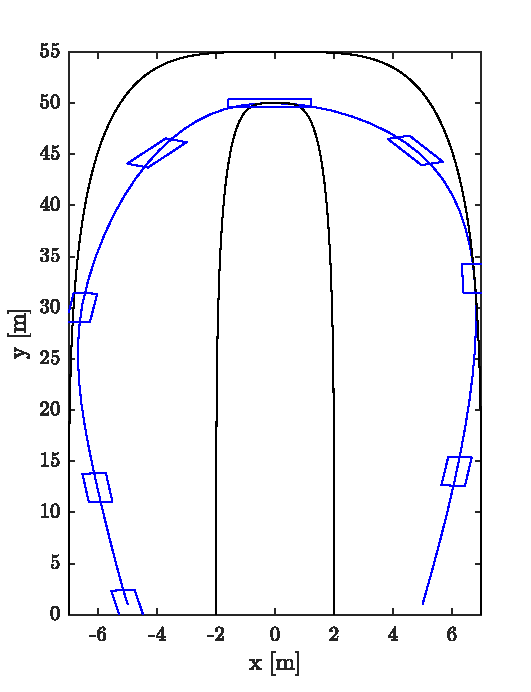
\includegraphics{figures/prob2_DT_path.pdf}
    \caption{Optimal trajectory for a harpin maneuver with minimum time for DT-model.}
    \label{fig:DT_hairpin_path}
\end{figure}

The states and forces acting on the wheels for the DT model for the hairpin are presented in Figure~\ref{fig:DT_hairpin_path_detail}. 

\begin{figure}[p]
    \centering
    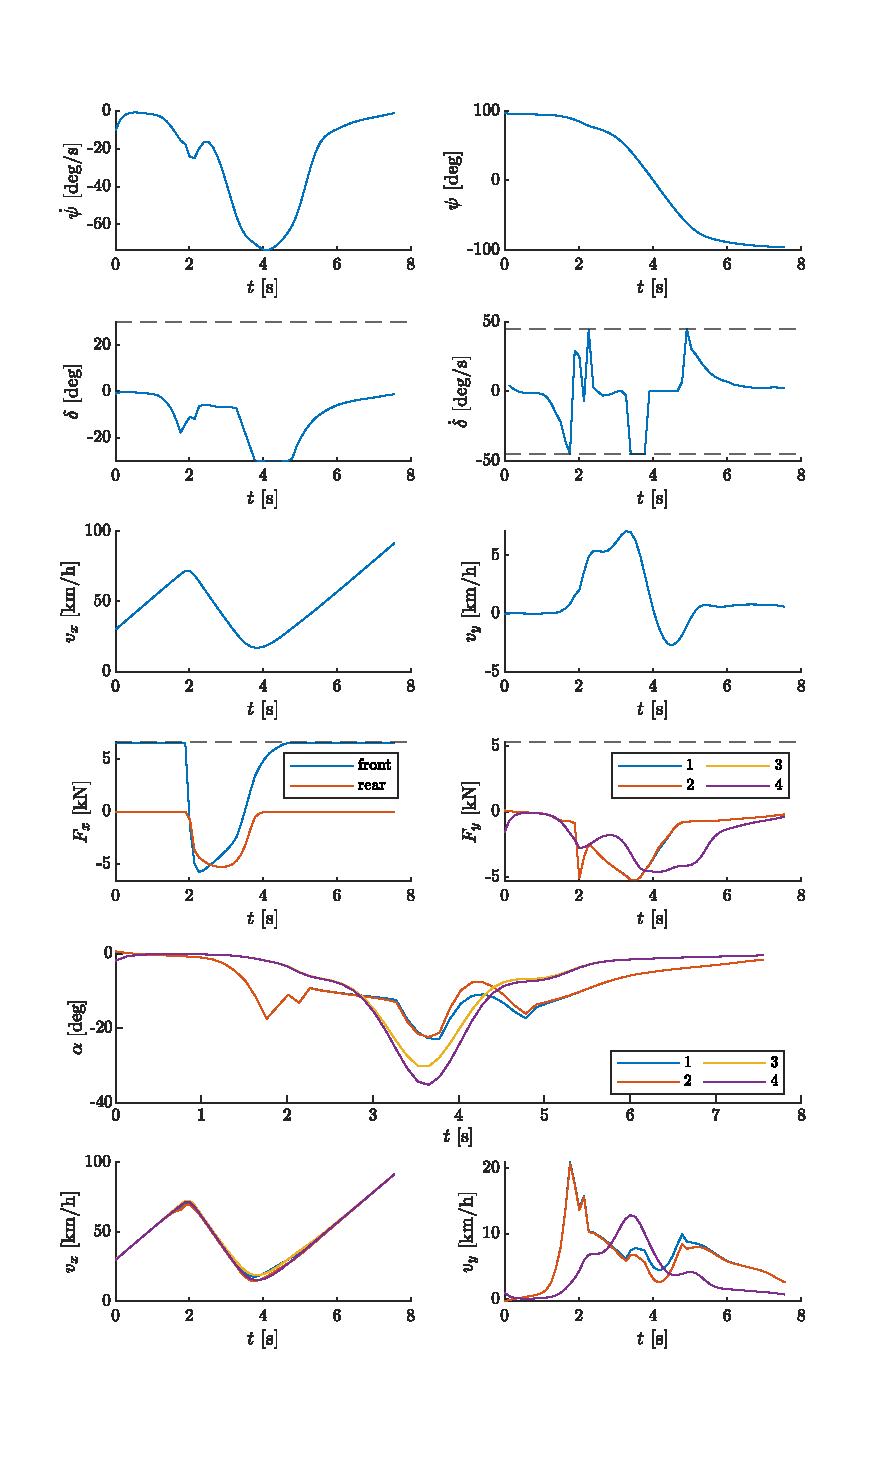
\includegraphics{figures/prob2_DT_path_detail.pdf}
    \caption{velocities, forces, and steering angels during the optimal trajectory for a harpin maneuver with minimum time for DT-model.}
    \label{fig:DT_hairpin_path_detail}
\end{figure}


\noindent\fbox{%
    \parbox{\textwidth}{%
        \textbf{Some reflections}: \newline
        The OCP for the DT model hairpin turn maneuver can have difficulty finding the optimal solution if the initial guesses are non-trivial. Therefore to improve convergence, the height of the hairpin was slowly increased, and the simulation results from the previous iterations were used as initializations for the next.
    }%
}

\section{Code}

The source code for this problem can be found at \newline \href{https://github.com/arvba41/optimal_vehicle_maneuvers/tree/main/uppgift/ugf2}{https://github.com/arvba41/optimal\_vehicle\_maneuvers}.

% $\mathbf{v_x > 0}$, to avoid $\div$ by zero error while calculating the lateral slips, $\alpha$.\\
% $\mathbf{-\delta_{max} \leq \delta \leq \delta_{max}}$, steering angle limit.\\
% $\mathbf{-\dot\delta_{max} \leq \dot\delta \leq \dot\delta_{max}}$, steering angle limit.\\
% opti.subject_to(-deltamax<=delta<=deltamax);    % steering angle limit
% opti.subject_to(-ddeltamax<=ddelta<=ddeltamax); % steering rate limit


\chapter{Verification of brake or evade criteria}

To verify the brake or evade criteria the following OCP was formulated:
\begin{align}
    & \underset{u}{\text{Min}}
    & & \mu\\
%
    & \text{subject to} 
    & & f_u(u) <= 0\\
%
    &&& \dot x = f(x,u),\\
%
    &&& x_0,\ x_f.
\end{align}

\section{Straight-line braking}
For straight-line braking, the following constraints are set up:
\begin{align}
    f_u(u): && 0 \geq F_x &\leq -F_{\text{max}} & F_y &= 0,\\
    \dot x = f(x,u): && \dot x &= v_x, & \dot y &= v_y, & \dot v_x &= \frac{F_x}{m}, & \dot v_y &= \frac{F_y}{m},\\
    x_0,\ x_f: && x(t_o) &= 0, & y(t_o) &= 0, & v_x(t_o) &= v_o, & v_y(t_o) &= 0,\\
    && x(t_f) &= x_f, & y(t_f) &= 0, & v_x(t_f) &= 0, & v_y(t_f) &= 0,
\end{align}
where $F_{\text{max}} = \mu m g$. The parameters of the vehicle are presented in Table~\ref{tab:brake_evade_params}.

The numerical verification for the break or evade criteria for straight-line braking is presented in Table~\ref{tab:brake_evade_straight_line_braking}.

\begin{table}[h!]
    \begin{subtable}{0.4\textwidth}
        \begin{tabular}{c|c}
            Parameters & Value \\
            \hline
            $m$ & 2000\,kg \\
            $g$ & 9.81\,m/s\textsuperscript{2} \\
        \end{tabular}
        \caption{Vehicle PM parameters.}
        \label{tab:brake_evade_params}
    \end{subtable}
    \hfill
    \begin{subtable}{0.6\textwidth}
        \begin{tabular}{c|c|c|c}
            & & Analytical & Simulation\\
            & $x_f$ & $\mu$ & $\mu$ \\
            % [m] & [-] & [m] & [-] \\
            \hline
            Dry Asphalt & 20.3\,m & 1 & 1.0043\\
            Wet Asphalt & 34\,m & 0.6 & 0.5996\\
            Ice Asphalt & 68\,m & 0.3 & 0.2998\\
        \end{tabular}
        \caption{Numerical and analytical solutions for road friction for straight-line braking with $v_0 = 20$\,m/s.}
        \label{tab:brake_evade_straight_line_braking}
    \end{subtable}
    \caption{Brake or evade for straight-line braking.} 
    \label{tab:brake_evade_straight}
\end{table}

\subsection{Code}
The source code for this problem can be found at \newline \href{https://github.com/arvba41/optimal_vehicle_maneuvers/blob/main/uppgift/ugf3/brake_or_evade_p1.m}{https://github.com/arvba41/optimal\_vehicle\_maneuvers}.

\section{Evading}
This section presents the numerical verification of evading criteria considering a PM.

\subsection{Wet asphalt maximum obstacle height}
To verify the largest obstacle that can be avoided without any braking on wet asphalt,the following OCP is formulated:
\begin{align}
    & \underset{u}{\text{Max}}
    & & & y(t_f)\\
%
    & \text{subject to} 
    & & & F_x &= 0 &0 \leq F_y &\leq F_{\text{max}},\\
%
    &&& & \dot x &= v_x, & \dot y &= v_y, & \dot v_x &= \frac{F_x}{m}, & \dot v_y &= \frac{F_y}{m},\\
%
    &&& & x(t_o) &= 0, & y(t_o) &= 0, & v_x(t_o) &= v_o, & v_y(t_o) &= 0,\\
    &&& & x(t_f) &= x_f,
\end{align}
where $F_{\text{max}} = \mu m g$, and the vehicle parameters are presented in Table~\ref{tab:brake_evade_params}.
\begin{table}[h!]
    \centering
    \begin{tabular}{c|c|c|c|c}
        & & & Analytical & Simulation\\
        $x_f$ & $v_0$ & $\mu$ & $y(t_f)$ & $y(t_f)$ \\
        % [m] & [-] & [m] & [-] \\
        \hline
        34\,m & 20\,m/s & 0.6 & 8.5\,m & 8.5053\,m \\
    \end{tabular}
    \caption{Numerical and analytical solutions for maximum obstacle height that a vehicle can avoid.}
\end{table}
\subsubsection{Code}
The source code for this problem can be found at \newline \href{https://github.com/arvba41/optimal_vehicle_maneuvers/blob/main/uppgift/ugf3/brake_or_evade_p2a.m}{https://github.com/arvba41/optimal\_vehicle\_maneuvers}.
\subsection{Minimum required friction}
To verify the minimum required friction to avoid an obstacle with a height of 1.7\,m at a distance of 34\,m, the following optimization problem was formulated:
\begin{align}
    & \underset{u}{\text{Min}}
    & & & \mu\\
%
    & \text{subject to} 
    & & & F_x &= 0 &0 \leq F_y &\leq F_{\text{max}},\\
%
    &&& & \dot x &= v_x, & \dot y &= v_y, & \dot v_x &= \frac{F_x}{m}, & \dot v_y &= \frac{F_y}{m},\\
%
    &&& & x(t_o) &= 0, & y(t_o) &= 0, & v_x(t_o) &= v_o, & v_y(t_o) &= 0,\\
    &&& & x(t_f) &= x_f, & y(t_f) &= y_f,
\end{align}
where $F_{\text{max}} = \mu m g$, and the vehicle parameters are presented in Table~\ref{tab:brake_evade_params}.
\begin{table}[h!]
    \centering
    \begin{tabular}{c|c|c|c|c}
        & & & Analytical & Simulation\\
        $x_f$ & $y_f$ & $v_0$ & $y(t_f)$ & $y(t_f)$ \\
        % [m] & [-] & [m] & [-] \\
        \hline
        34\,m & 1.7\,m & 20\,m/s & 0.12 & 0.1199 \\
    \end{tabular}
    \caption{Numerical and analytical solutions for the minimum required friction to avoid an obstacle.}
\end{table}
\subsubsection{Code}
The source code for this problem can be found at \newline \href{https://github.com/arvba41/optimal_vehicle_maneuvers/blob/main/uppgift/ugf3/brake_or_evade_p2b.m}{https://github.com/arvba41/optimal\_vehicle\_maneuvers}.
\subsection{Minimum distance to object}
To verify the minimum distance to an object with a height of 1.7\,m on wet asphalt, the following optimization problem was formulated:
\begin{align}
    & \underset{u}{\text{Max}}
    & & & x(t_f)\\
%
    & \text{subject to} 
    & & & F_x &= 0 &0 \leq F_y &\leq F_{\text{max}},\\
%
    &&& & \dot x &= v_x, & \dot y &= v_y, & \dot v_x &= \frac{F_x}{m}, & \dot v_y &= \frac{F_y}{m},\\
%
    &&& & x(t_o) &= 0, & y(t_o) &= 0, & v_x(t_o) &= v_o, & v_y(t_o) &= 0,\\
    &&& & y(t_f) &= y_f,
\end{align}
where $F_{\text{max}} = \mu m g$, and the vehicle parameters are presented in Table~\ref{tab:brake_evade_params}.
\begin{table}[h!]
    \centering
    \begin{tabular}{c|c|c|c|c}
        & & & Analytical & Simulation\\
        $\mu$ & $y_f$ & $v_0$ & $x(t_f)$ & $x(t_f)$ \\
        % [m] & [-] & [m] & [-] \\
        \hline
        0.6 & 1.7\,m & 20\,m/s & 15.2\,m & 15.2006\,m\\
    \end{tabular}
    \caption{Numerical and analytical solutions for the maximum distance to an obstacle that can be avoided.}
\end{table}
\subsubsection{Code}
The source code for this problem can be found at \newline \href{https://github.com/arvba41/optimal_vehicle_maneuvers/blob/main/uppgift/ugf3/brake_or_evade_p2c.m}{https://github.com/arvba41/optimal\_vehicle\_maneuvers}.
\chapter{Numerical solution of optimal avoidance for PM}
To determine the numerical solution of optimal avoidance for PM, the following OCP is formulated:
\begin{align}
    & \underset{F_x,\ F_y}{\text{Min}}
    & & & \mu\\
%
    & \text{subject to} 
    & & & F_x &\leq 0 & 0 &\leq F_y & F_x^2 + F_y^2 &\leq F_{\text{max}}^2,\\
%
    &&& & \dot x &= v_x, & \dot y &= v_y, & \dot v_x &= \frac{F_x}{m}, & \dot v_y &= \frac{F_y}{m},\\
%
    &&& & x(t_o) &= 0, & y(t_o) &= 0, & v_x(t_o) &= v_o, & v_y(t_o) &= 0,\\
    &&& & x(t_f) &= \text{A}+25, \\
    &&& & f_o(x,y) &>= 1 ,
\end{align}
where 
\begin{equation}
    f_o(x,y) = \left(\frac{x-\text{A}}{R_1}\right)^n + \left(\frac{y}{R_2}\right)^n
\end{equation}
is the obstacle, $F_{\text{max}} = \mu m g$, and the vehicle parameters are presented in Table~\ref{tab:num_sol_opt_avoid_PM_params}.
\begin{table}[h!]
    \begin{subtable}{0.38\textwidth}
        \begin{tabular}{c|c}
            \multicolumn{2}{c}{Vehicle} \\
            \hline
            $m$ & 2000\,kg \\
            $g$ & 9.81\,m/s\textsuperscript{2} \\
            \multicolumn{2}{c}{Obstacle} \\
            \hline
            $R_1$ & 5 \\
            $R_2$ & 3 \\
            $n$ & 20 \\
        \end{tabular}
        \caption{Vehicle PM and obstacle parameters.}
        \label{tab:num_sol_opt_avoid_PM_params}
    \end{subtable}
    \hfill
    \begin{subtable}{0.58\textwidth}
        \begin{tabular}{c|c|c|c}
            & & Analytical & Simulation\\
            A & B & $\mu$ & $\mu$ \\
            % [m] & [-] & [m] & [-] \\
            \hline
            20.5047\,m & 2.9012\,m & 0.5546 & 0.5583
        \end{tabular}
        \caption{Numerical and analytical solutions for minimum road friction for optimal obstacle with $v_0 = 20$\,m/s.}
        \label{tab:num_sol_opt_avoid_PM_res}
    \end{subtable}
    \caption{Brake or evade for straight-line braking.} 
    \label{tab:num_sol_opt_avoid_PM}
\end{table}

\section{Analytical solution}
The analytical solution is determined by first calculating $\gamma$, 
\begin{align}
    \gamma &= \arctan\left(\frac{\text{B}}{\text{A}}\right),
\end{align}
where B and A are the height and distance of the obstacle and the trajectory intersection point, assuming that the vehicle is starting from (0,0). 
$\theta$ is calculated using the relation
\begin{align}
    \theta &= \frac{\gamma + \arcsin\left(3\sin\left(\gamma\right)\right)}{2}.
\end{align}
Now, $\mu$ is calculated using 
\begin{align}
    \mu &= \frac{2\sin\left(2\gamma\right)\cos\left(\theta\right)}{\cos\left(\theta-\gamma\right)^2}\frac{v_o^2}{2g\text{A}}.
\end{align}
The comparison between the optimal and analytically calculated $\mu$ is presented in Table~\ref{tab:num_sol_opt_avoid_PM_res}.

\section{Code}
The source codes for this problem can be found at \newline \href{https://github.com/arvba41/optimal_vehicle_maneuvers/blob/main/uppgift/ugf4/opti_veh_men_prt.m}{https://github.com/arvba41/optimal\_vehicle\_maneuvers}.

The detailed results of the optimization problem are presented in Figure~\ref{fig:num_sol_opt_avoid_PM_res_pic}.
\begin{figure}[h!]
    \centering
    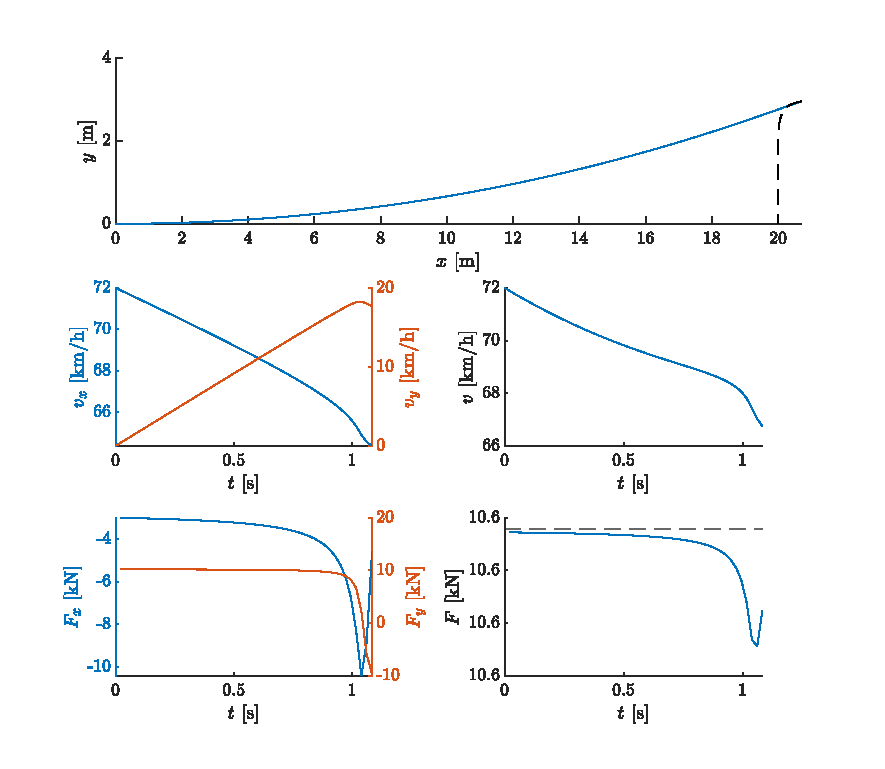
\includegraphics{figures/prob4_opt_avoid_path.pdf}
    \caption{Numerical solution for the optimal obstacle avoidance.}
    \label{fig:num_sol_opt_avoid_PM_res_pic}
\end{figure}

\chapter[Force and scenario centric]{Avoidance with criterion max $F_{c,y}$ as an exercise with both a scenario-centric and a force-centric perspective}

To determine the avoidance with criterion max $F_{c,y}$ (force (control force) centric) and $F_{Y}$ (vehicle centric),  OCPs with the following cost functions are formulated:
\begin{align}
    \text{Min}\ t & \quad\text{topt}\\
    \text{Max}\ \int_{t_s}^{t_f} F_{c,y}(t) dt & \quad\text{Fcopt}\\
    \text{Max}\ \int_{t_s}^{t_f} F_{Y}(t) dt & \quad\text{Fyopt}
        % \text{Min}\ t & \text{topt}\\
        % \text{Max}\ \int_{t_s}^{t_f} F_{c(y)} dt & \text{Fcopt}\\
        % \text{Max}\ \int_{t_s}^{t_f} F_{Y} dt & \text{Fyopt}
\end{align}

A double track (DT) model is used with $F_{x(i)}$ as the control inputs, where $i = 1,\ 2,\ 3,\ 4$, and 
\begin{align}
    \begin{array}{cl}
        F_{x(1)} = F_{x(2)} = F_{x(f)}, & -F_{f(\text{max})} \leq F_{x(f)} \leq F_{f(\text{max})}, \\
        F_{x(3)} = F_{x(4)} = F_{x(r)}, & -F_{r(\text{max})} \leq F_{x(f)} \leq 0,
    \end{array}
\end{align}
where $F_{f(\text{max})}$ and $F_{r(\text{max})}$ are detemined using 
\begin{align}
    F_{f(\text{max})} &= \mu_{x(f)}F_{z(f)}, & F_{r(\text{max})} &= \mu_{x(r)}F_{z(r)},
\end{align}
and $F_{z(f)}$, $F_{z(r)}$ are determined using \eqref{eq:prob2_maxforce_DT}.

The obstacle is given by the following relation, 
\begin{align}
    \left(\frac{x - X_a}{R_1}\right)^n + \left(\frac{y}{R_2}\right)^n \geq 1,
\end{align}
A dimensionless parameter $\gamma$ is calculated using 
\begin{align}
    \gamma &= \arctan\left(\frac{B}{A}\right), & B &= R_2, & A&= X_a - R_1.
\end{align}
This is rather conservative and aids the vehicle to avoid the obstacle. 
$\gamma$, in this case, is 9.5$^\circ$ ($\geq 16.7^\circ$), and considering wet asphalt (see \ref{sec:prob3_STrbrk}), then evading is a better option. 
It is worth mentioning that $\gamma$ is calculated using the obstacle height rather than the lateral distance where the vehicle and the obstacle intersect. 
This is to provide a better chance for the vehicle to avoid the obstacle. 

The angle of the obstacle ($\theta_v$) is the angle between the component of the global force ($F_{x}$) and the velocity vector and is calculated using 
\begin{align}
    \theta_v = \frac{\gamma + \arcsin\left(3\sin\left(\gamma\right)\right)}{2}.
\end{align}
The control force vectors ($F_{c,x}$ and $F_{c,y}$) are calculated using
\begin{align}
    \begin{bmatrix}
        F_{c,x}(t) \\
        F_{c,y}(t)
    \end{bmatrix} &=
    \begin{bmatrix}
        \cos\left(\theta_v\right) & \sin\left(\theta_v\right) \\
        -\sin\left(\theta_v\right) & \cos\left(\theta_v\right)
    \end{bmatrix}
    \begin{bmatrix}
        \cos\left(\psi(t)\right) & -\sin\left(\psi(t)\right) \\
        \sin\left(\psi(t)\right) & \cos\left(\psi(t)\right)
    \end{bmatrix}
    \begin{bmatrix}
        F_{X}(t)\\
        F_{Y}(t)
    \end{bmatrix}.
\end{align}

A solution to the optimization problem is determined using the homotopic approach. The OCP is solved for the topt case and this solution is used as initial guesses for Fcopt and Fyopt. 

The constraints to the optimization problem are 
\begin{align}
    \begin{array}{ccccc}
        |\delta| \leq \delta_\text{max} & |\dot\delta| \leq \dot\delta_\text{max} & 
        0 \leq t \leq t_{\text{max}} & 0 \leq y \leq y_\text{max} & 0 \leq x \leq x_\text{max}
    \end{array}
\end{align}

\begin{table}[h!]
    \centering
    \begin{subtable}{0.3\textwidth}
        \begin{tabular}{c|c}
            Parameter & Value\\
            \hline
            $X_a$ & 20\,m\\
            $R_1$ & 2\,m\\
            $R_2$ & 3\,m\\
            $n$ & 12
        \end{tabular}
        \caption{Obstacle parameters}
        \label{tab:obst_pprty}
    \end{subtable}
    \begin{subtable}{0.3\textwidth}
        \begin{tabular}{c|c}
            Parameter & Value\\
            \hline
            $m$ & 2100\,kg\\
            $l_f$ & 1.3\,m\\
            $l_r$ & 1.5\,m\\
            $w$ & 0.8\,m\\
            $g$ & 9.81\,m/s\textsuperscript{2}\\
            $I_{zz}$ & 3900\,kg\textsuperscript{2}
        \end{tabular}
        \caption{Vehicle parameters}
        \label{tab:veh_pprty}
    \end{subtable}
    \begin{subtable}{0.3\textwidth}
        \begin{tabular}{c|c}
            Parameter & Value\\
            \hline
            $\delta_\text{max}$ & 30$^\circ$\\
            $\dot\delta_\text{max}$ & 45$^\circ$/s\\
            $v_x(t_0)$ & 20\,m/s\\
            $t_{\text{max}}$ & 2\,s\\
            $y_{\text{max}}$ & 7.5\,m\\
            $y_{\text{max}}$ & 20\,m\\
            $y(t_f)$ & 3\,m
        \end{tabular}
        \caption{Optimization constraints}
        \label{tab:const_pprty}
    \end{subtable}
    \caption{Obstacle-, vehicle-parameters and optimization constrains.}
\end{table}

The optimal trajectories for the three OCPs are shown in Figure~\ref{fig:prob6_traj}. From the figure, it is clear that the trajectories for the three cases are similar. An expected solution should be that the Fcopt and Fyopt solution avoids the obstacle with some room to spare. It is difficult to say why this is happening. However, a clue is when comparing the solution of Fcyopt and OCP solution with the cost function to maximize the input velocity (vopt). In this case, the vopt and Fcopt should have identical trajectories and this is shown in Figure~\ref{fig:prob6_v2_traj}. 
\begin{figure}[h!]
    \centering
    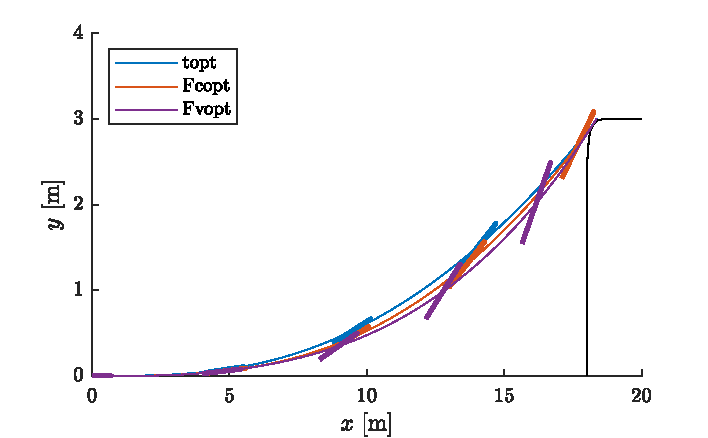
\includegraphics{figures/prob6_traj.pdf}
    \caption{Trajectories for time (topt), control force centric (Fcopt), and vehicle centric (Fyopt) optimal obstacle avoidance maneuver. The rectangles indicate the position and orientation of the vehicle every 0.25\,s.}
    \label{fig:prob6_traj}
\end{figure}
\begin{figure}[t!]
    \centering
    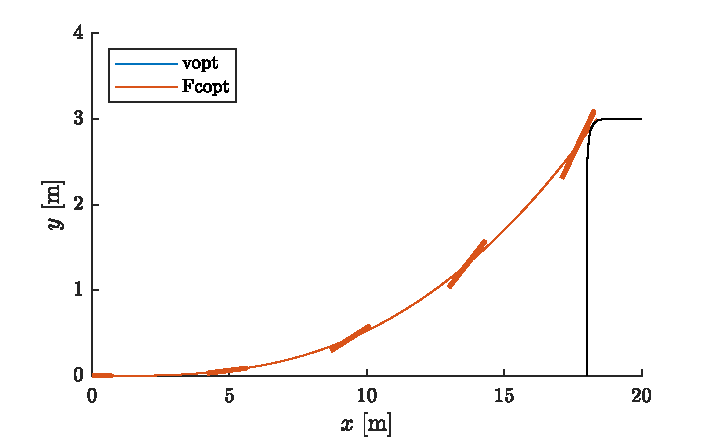
\includegraphics{figures/prob6_v2_traj.pdf}
    \caption{Trajectories for input velocity (vopt) and control force centric (Fcopt) optimal obstacle avoidance maneuver. The rectangles indicate the position and orientation of the vehicle every 0.25\,s.}
    \label{fig:prob6_v2_traj}
\end{figure}
\clearpage
The forces are shown in Figure~\ref{fig:prob6_forces}. From the figure, $F_{c,y}$ is maximized at every time instant for the Fcopt case. At $x = 5$\,m, $F_{c,y}$ for topt is greater than Fcopt because $|F_{c,x}|$ for topt is lower than for Fcopt. Figure~\ref{fig:prob6_detailed} shows the vehicle model variables for all the there OCPs. From the figure, it can be seen that the velocity for the topt stays constant. In the Fopt case, the velocity reduces significantly until 15\,m (as the vehicle approaches the object and $\varphi_v(t) \rightarrow \theta_v$), and then the rate of change of velocity reduces. The lateral slips for the Fyopt case are the highest because Fy is maximized at every time instant. The lateral forces on the wheels for Fcopt and Fyopt are similar until 15\,m and as the vehicle approaches the obstacle ($\varphi_v(t) \rightarrow \theta_v$), in Fcopt, $F_Y$ starts to reduce and $F_X$ starts to increase. However, Fyopt tries to make the vehicle go around in circles. 

\begin{figure}[h]
    \centering
    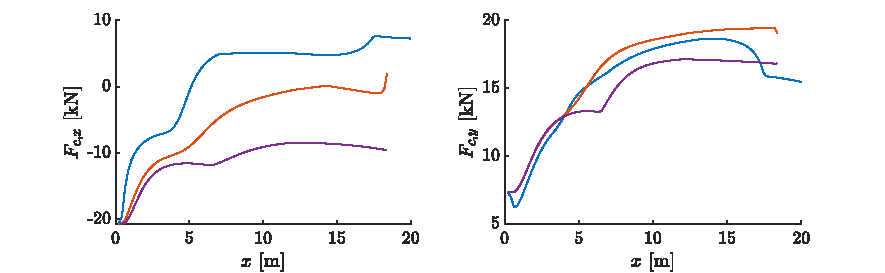
\includegraphics{figures/prob6_forces.pdf}
    \caption{Control forces for the time (topt), control force centric (Fcopt), and vehicle centric (Fyopt) optimal obstacle avoidance maneuver.}   
    \label{fig:prob6_forces}
\end{figure}

\begin{figure}[h]
    \centering
    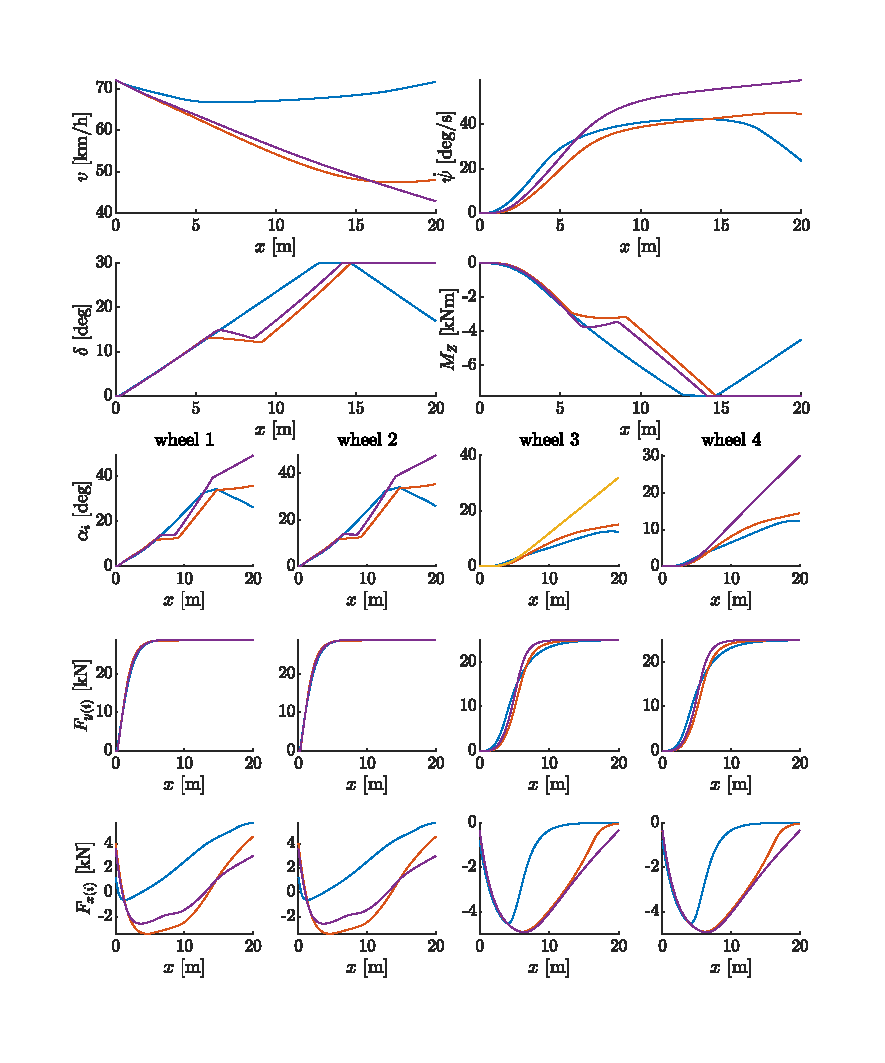
\includegraphics{figures/prob6_detailed.pdf}
    \caption{Variables of the vehicle model during the time (topt), control force centric (Fcopt), and vehicle centric (Fyopt) optimal obstacle avoidance maneuver.}   
    \label{fig:prob6_detailed}
\end{figure}

\noindent\fbox{%
    \parbox{\textwidth}{%
        \textbf{Some reflections}: \newline
        While analyzing the results, for some reason, $F_Y$ is negative, and $F_X$ seems to be similar for all three cases and the reason for this is unknown. Probably this is some bug in the model that can be fixed for future versions. \newline
        I was expecting the trajectories for the Fcopt and Fyopt solutions to avoid the obstacle with a significant distance to the vehicle. When the optimization was rerun with a free value for the initial velocity, then this is observed. However, the initial velocities for the three OCPs are different, especially for Fvopt. The solver struggles to converge to a solution and often throws a restoration failed error message. A homotopic approach can be used to guide ipopt in the desired direction. 
    }
}



% \section{The particle model}
% The angle of the obstacle ($\psi_v$) is the angle between the component of the global force ($F_{x}$) and the velocity vector and is calculated using 
% \begin{align}
%     \psi_v(t) &= \frac{dy(t)}{dx(t)}.
% \end{align}
% The vehicle centric control force vectors ($F_{c,x}$ and $F_{c,y}$) are calculated using
% \begin{align}
%     \begin{bmatrix}
%         F_{v,x}(t) \\
%         F_{v,y}(t)
%     \end{bmatrix} &=
%     \begin{bmatrix}
%         \cos\left(\psi_v(t)\right) & \sin\left(\psi_v(t)\right) \\
%         -\sin\left(\psi_v(t)\right) & \cos\left(\psi_v(t)\right)
%     \end{bmatrix}
%     \begin{bmatrix}
%         F_{x}(t)\\
%         F_{y}(t)
%     \end{bmatrix}.
% \end{align}
% $\psi_v$ when the vehicle just touches the obstacle at time $t_o$ is calculated using 
% \begin{align}
%     \theta &= \psi_v(t_o)\vert_{f_o(x,y)=1}.
% \end{align}
% The scenario centric control force vectors ($F_{c,x}$ and $F_{c,y}$) are calculated using
% \begin{align}
%     \begin{bmatrix}
%         F_{c,x}(t) \\
%         F_{c,y}(t)
%     \end{bmatrix} &=
%     \begin{bmatrix}
%         \cos\left(\theta\right) & \sin\left(\theta\right) \\
%         -\sin\left(\theta\right) & \cos\left(\theta\right)
%     \end{bmatrix}
%     \begin{bmatrix}
%         F_{x}(t)\\
%         F_{y}(t)
%     \end{bmatrix}.
% \end{align}

% The optimization results for the force and scenario centric are presented in Figure~\ref{fig:prob5_res}. From the figure, it is clear that the control force magnitude for the $y$ direction is constant for both the scenario-, vehicle-, and global-centric. However, the $x$ is different for scenarios, which is rather intuitive.

% \vspace{5pt}
% \noindent\fbox{%
%     \parbox{\textwidth}{%
%         \textbf{Some reflections}: \newline
%         It is worth mentioning that, in Figures~\ref{fig:num_sol_opt_avoid_PM_res_pic} and ~\ref{fig:prob5_res}, the intersection occurs at $t = 1.07$s. However, the vehicle starts to decelerate in the $y$-direction at around 1\,s, when $x = 20$\,m. This is probably due to the order of sharpness of the obstacle. when the degree of the super ellipse (obstacle model) is reduced, the vehicle starts to decelerate earlier and smoother. 
%     }%
% }

% \begin{figure}[h!]
%     \centering
%     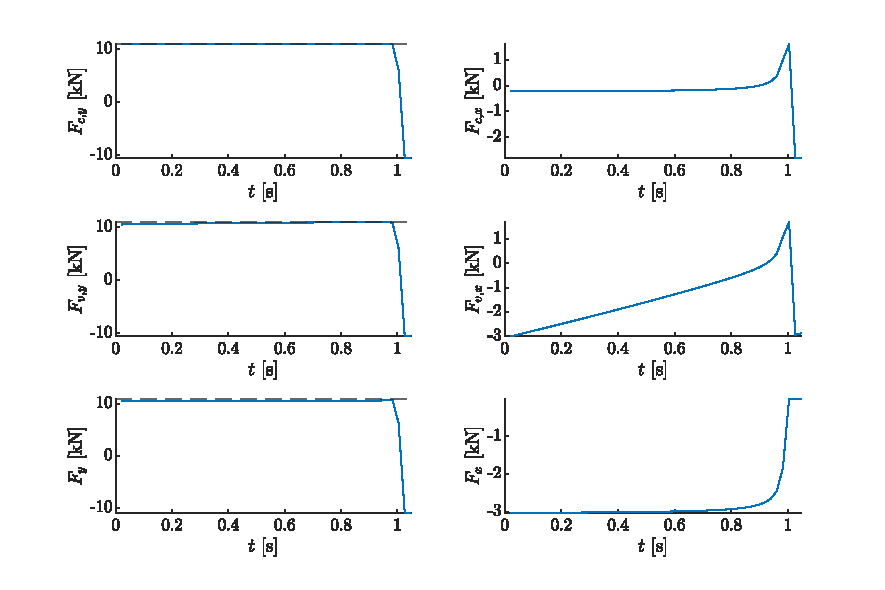
\includegraphics{figures/prob5_opt_avoid_controlforce.pdf}
%     \caption{Criteria for max $F_{c,y}$ for both a scenario-centric and a force-centric perspective.}
%     \label{fig:prob5_res}
% \end{figure}

\subsection{Code}
The source codes for this problem can be found at \newline \href{https://github.com/arvba41/optimal_vehicle_maneuvers/blob/main/uppgift/ugf5/force_centric_and_scenario_centric_PM.m}{https://github.com/arvba41/optimal\_vehicle\_maneuvers}.
\chapter[PEP: Pundilum Turn]{The pendulum turn: Are many rally drivers wrong?}

Well, Maybe! To answer this question two optimization problems (OCPs) were formulated. One OCP was to minimize the time and the other to maximize the exit velocity. Section~\ref{sec:STM} in the chapter presents the ST model and Section.. presents the constraints. In Section... the parameters of the model are presented. Finally, the results are presented in Section.

\section[ST model]{Single track model}\label{sec:STM}
In an earth-fixed coordinate system, the position ($X_p,\ Y_p$) and orientation of the vehicle is obtained from the differential equations
\begin{subequations}
    \begin{align}
        \dot X_p &= v_x\cos\left(\psi\right) - v_y\sin\left(\psi\right), \\
        \dot Y_p &= v_x\sin\left(\psi\right) + v_y\cos\left(\psi\right), \\
        \dot \psi &= r.
    \end{align}
\end{subequations}
The longitudinal and lateral velocities and yar rate are given by the following differential equations 
\begin{subequations}
    \begin{align}
        \dot v_x &= \frac{F_X}{m} + v_y\,r,\\
        \dot v_y &= \frac{F_Y}{m} - v_x\,r,\\
        \dot v_y &= \frac{M_Z}{I_{zz}},
    \end{align}
\end{subequations}
where 
\begin{subequations}
    \begin{align}
        F_X &= F_{x(f)}\cos\left(\delta\right) - F_{y(f)}\sin\left(\delta\right) + F_{x(r)},\\
        F_Y &= F_{x(f)}\sin\left(\delta\right) + F_{y(f)}\cos\left(\delta\right) + F_{y(r)},\\
        M_Z &= l_f\left(F_{x(f)}\sin\left(\delta\right) + F_{y(f)}\cos\left(\delta\right)\right) - l_rF_{y(r)},
    \end{align}
\end{subequations}
where $\delta$ is the steering angle and $\dot \delta$ is an input to the model. Furthermore, 
\begin{subequations}
    \begin{align}
        F_{x(f)} = \frac{1}{\tau_f}\left(F_{x(f)}^* - F_{x(f)}\right),\\
        F_{x(r)} = \frac{1}{\tau_f}\left(F_{x(r)}^* - F_{x(r)}\right),
    \end{align}
\end{subequations}
where $F_{x(f)}^*$, and $F_{x(r)}^*$ are the inputs to the model, and $\tau_f$ is the filter time constant. 

A simple model for combined slip is the friction-ellipses-based combined-slip model is used and is given as
\begin{align}
    F_{y(f)} &= F_{y0(f)}\sqrt{1 - \left(\frac{F_{x(f)}}{F_{x0(f)}^{\text{max}}}\right)} & F_{y(r)} &= F_{y0(r)}\sqrt{1 - \left(\frac{F_{x(r)}}{F_{x0(r)}^{\text{max}}}\right)},
\end{align}
where 
\begin{align}
    F_{x0(f)}^{\text{max}} &= \mu_{x(f)}F_{z(f)} & F_{x0(r)}^{\text{max}} &= \mu_{x(r)}F_{z(r)},\\
    F_{z(f)} &= \frac{mgl_r}{l_f+ l_r} & F_{z(r)} &= \frac{mgl_f}{l_f+ l_r}.
\end{align}
Pacejka's Magic Formula model is used to determine the pure slips, $F_{y0(f)},\ F_{y0(r)}$.
\section{Optimization procedure}\label{sec:STcons}
The constraints on the optimization problems are as follows:
\begin{subequations}
    \begin{align}
        -\delta_{\text{max}} &\leq \delta \leq \delta_{\text{max}},\\
        -\dot\delta_{\text{max}} &\leq \dot\delta \leq \dot\delta_{\text{max}},\\
        -F_{x(f),\text{max}} &\leq F_{x(f)} \leq F_{x(f),\text{max}},\\
        -F_{x(r),\text{max}} &\leq F_{x(r)} \leq 0,\\
        -F_{x(f),\text{max}} &\leq F_{x(f)}^* \leq F_{x(f),\text{max}},\\
        -F_{x(r),\text{max}} &\leq F_{x(r)}^* \leq 0,\\
        v_x &> 0\\
        0 &\leq \beta_x \leq 1\\
        0 &\leq \beta_y \leq 1,
    \end{align}
\end{subequations}
where $F_{x(i),\text{max}} = \mu_{x(i)}\,F_{z(i)}$. The limits are presented in Table~\ref{tab:st_const}. $\beta_x,\ \beta_y$ are slack variables. 

The hairpin is given by
\begin{align}
    \left(\frac{x-X_\text{a}}{R_1^i}\right)^n + \left(\frac{y}{R_2^i}\right)^n & \geq 1, & \left(\frac{x-X_a}{R_1^o}\right)^n + \left(\frac{y}{R_2^o}\right)^n & \leq 1.
\end{align}

The path to finding the optimal solution was not easy. The OCP was reduced to a hairpin with just 1\,m height with the initial conditions presented as in Table~\ref{tab:st_guess}. Then the height was gradually increased to 50\,m, and the solution of the previous solution is used as an initial guess. To increase computation time, slack variables ($\beta_x,\ \beta_y$) on the final positions are introduced. 

\begin{table}[h!]
    \begin{subtable}{0.3\textwidth}
        \begin{tabular}{c|c}
            Parameter & Value \\
            \hline
            $\delta_{\text{max}}$ & 30$^\circ$ \\
            $\dot \delta_{\text{max}}$ & 45$^\circ$/s\\
            $\tau_f$ & 0.1\,s\\
            $X_a$ & 10\,m\\
            $R_1^i$ & 2\,m\\
            $R_2^i$ & 50\,m\\
            $R_1^o$ & 7\,m\\
            $R_2^o$ & 55\,m\\
            $n$ & 4\\
        \end{tabular}
        \caption{Constraints on the optimization problem.}
        \label{tab:st_const}
    \end{subtable}
    \hfill
    \begin{subtable}{0.3\textwidth}
        \begin{tabular}{c|c}
            Parameter & Value \\
            \hline
            $X_p(t_0)$ & 5\,m\\
            $Y_p(t_0)$ & 0\,m\\
            $X_p(t_f)$ & 14 + $\beta_x$\,m\\
            $Y_p(t_f)$ & 0 + $\beta_y$\,m\\
            $v_x(t_0)$ & 30\,km/h\\
            $v_y(t_0)$ & 0\,km/h\\
            $F_{x(f)}(t_0)$ & 0\,N\\
            $F_{x(r)}(t_0)$ & 0\,N\\
        \end{tabular}
        \caption{Initial conditions to the optimization problem.}
        \label{tab:st_init}
    \end{subtable}
    \hfill
    \begin{subtable}{0.3\textwidth}
        \begin{tabular}{c|c}
            Parameter & Value \\
            \hline
            $\psi$ & 0$^\circ$\\
            $v_x$ & 30\,km/h\\
            $v_x$ & 0\,km/h\\
            $r$ & 0$^\circ$/s\\
            $\delta$ & 0$^\circ$\\
            $\dot \delta$ & 0$^\circ$/s\\
            $t_f$ & 10\,s\\
            $F_{x(f)}^*$ & 0\,N\\
            $F_{x(r)}^*$ & 0\,N\\
        \end{tabular}
        \caption{Initial guess for the optimization problem with the hairpin height of 1\,m.}
        \label{tab:st_guess}
    \end{subtable}
    \caption{Optimization parameters and constraints.}
\end{table}

The cost function is given by
\begin{align}
    J &= \begin{cases} 
            \text{Min }\quad t + 0.1\left(\beta_x + \beta_y\right) & \text{min } t \\
            \text{Max }\quad v_x(t_f) + 0.1\left(\beta_x + \beta_y\right) & \text{max } v_f 
         \end{cases}.
\end{align}
\section{Parameters}\label{sec:STparams}
The parameters for the model are presented in Table~\ref{tab:mgtire_params}.
\begin{table}[h!]
    \begin{subtable}{0.49\textwidth}
        \begin{tabular}{c|c|c}
            Parameter & Front & Rear \\
            \hline
            $\mu_x$ & 1.2 & 1.2\\
            $B_x$ & 11.7 & 11.1\\
            $C_x$ & 1.67 & 1.69\\
            $E_x$ & 0.377 & 0.362\\
            $\mu_y$ & 0.935 & 0.961\\
            $B_y$ & 8.86 & 9.30\\
            $C_y$ & 1.19 & 1.19\\
            $E_y$ & -1.21 & -1.11\\
        \end{tabular}
        \caption{Pacejka Magic Formula model parameters.}
        \label{tab:mgtire_params}
    \end{subtable}
    \hfill
    \begin{subtable}{0.49\textwidth}
        \begin{tabular}{c|c}
            Parameter & Value\\
            \hline
            $m$ & 2100\,kg\\
            $l_f$ & 1.3\,m\\
            $l_r$ & 1.5\,m\\
            $g$ & 9.82\,m/s\textsuperscript{2}\\
            $I_{zz}$ & 3900\,kgm\textsuperscript{2}\\
        \end{tabular}
        \caption{Vehicle model parameters.}
        \label{tab:veh_ST_params}
    \end{subtable}
    \caption{Model parameters.}
\end{table}

\section{Reults}
This section presents the optimal trajectory for the two OCPs: minimum time to complete the maneuver, and maximum exit velocity from the hairpin. The results are shown in Figures~\ref{fig:pep1_part1} and~\ref{fig:pep1_part1_arp}.

\begin{figure}[h!]
    \centering
    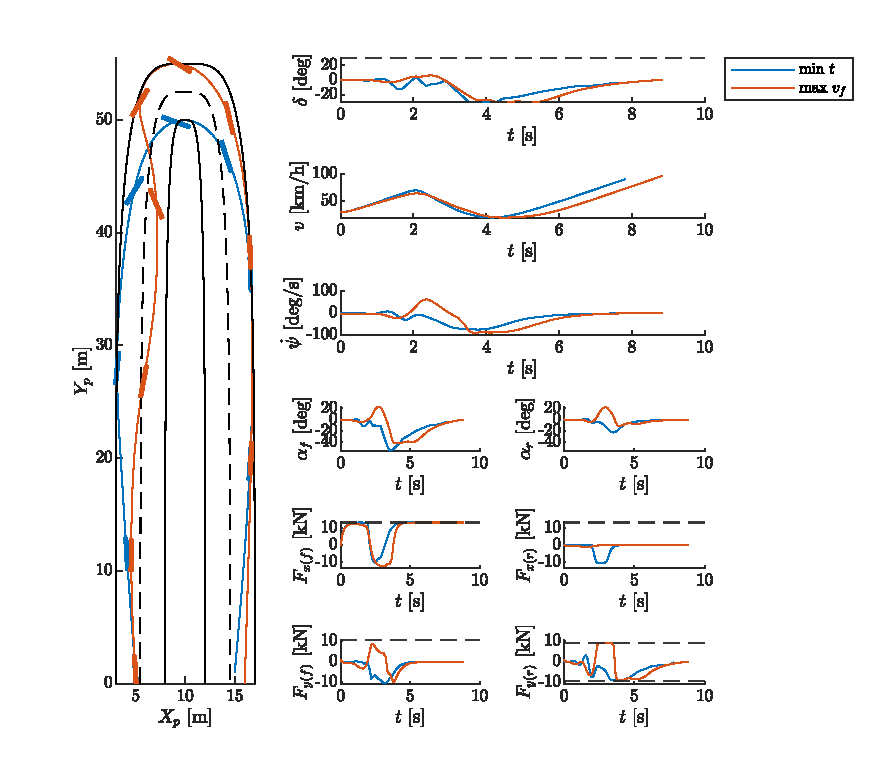
\includegraphics{figures/pep1_part1.pdf}
    \caption{Time and velocity optimized trajectories for the ST model through a hairpin.}
    \label{fig:pep1_part1}
\end{figure}

\begin{figure}[h!]
    \centering
    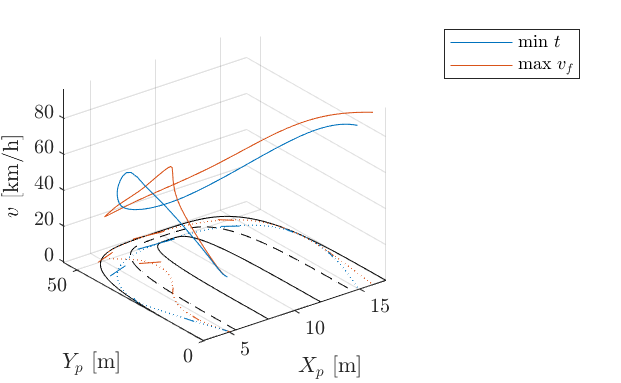
\includegraphics{figures/pep1_part1_arp.pdf}
    \caption{Optimal trajectory and speed profile for time and velocity optimized trajectories for the ST model through a hairpin.}
    \label{fig:pep1_part1_arp}
\end{figure}

The results of the final time and speed for the two optimization problems (Min $t$, and Max $v_f$) at the end of the maneuver are summarized in Table~\ref{tab:opt_res_num_pep1}. 
From the table, it is clear that at $Y_o = 0$, Case-V (pendulum turn case) is about 1.5\,m/s faster but takes about 1\,s more to complete the maneuver. 
\begin{table}[h!]
    \centering
    \begin{tabular}{c|c|c|c}
        & & $t_f$ & $v_f$\\
        \hline
        \textbf{Case-T:} & Min $t_f$ & 7.83\,s & 25.11 m/s (90.4\,km/h)\\
        \textbf{Case-V:} & Max $v_f$ & 8.84\,s & 26.68 m/s (96\,km/h)\\
    \end{tabular}
    \caption{Time and speed for the ST model for the two optimization cases T and V at the end of maneuver, $Y_o = 0$.}
    \label{tab:opt_res_num_pep1}
\end{table}

Consider Figure~\ref{fig:opt_res_num_pep1}, assuming that the vehicles in both cases are traveling side-by-side, then the vehicle in case-V will begin to overtake case-T at distance $Y_i$. Since the time taken to complete the maneuver are different for the two cases, the vehicle in case-T would have reached $Y_{T0}$ during the time duration, $\delta t$. 
\begin{figure}[h!]
    \centering
    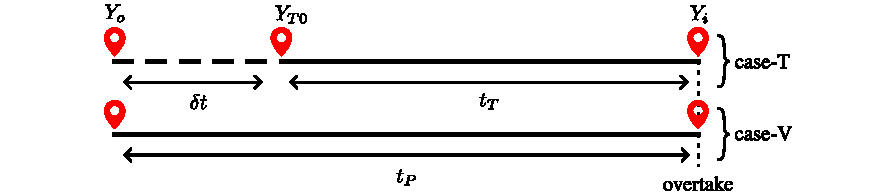
\includegraphics{figures/pep1_analys.pdf}
    \caption{Vehcile trajectories after the maneuver.}
    \label{fig:opt_res_num_pep1}
\end{figure}

$Y_{T0}$ and the speed at $Y_{T0}$, $v_{T0}$, assuming the same acceleration for both the vehicles from $Y_o$ to $Y_i$, is calculated by
\begin{align}
    Y_{T0} &= \frac{\mu g\left(\delta t\right)^2}{2} +  V_{y0(T)}\delta t + Y_o, & v_{T0} &= \mu g\delta t +  V_{y0(T)}.
\end{align}

For the intersection of the two cases to be even possible, 
\begin{align}
    v_{T0} &\leq V_{yo(V)}, & \mu g\delta t +  V_{y0(T)} &\leq V_{yo(V)},
\end{align}
where $V_{yo(V)}$ is the velocity at the end of the maneuver for case-V. 

For the intersection to be feasible, 
\begin{align}
    \mu &\leq \frac{V_{yo(V)} - V_{y0(T)}}{g\delta t}.\label{eq:mdl1}
\end{align}
Substituting the values of $g$, $\delta t$, $V_{yo(V)}$, and $V_{y0(T)}$ in \eqref{eq:mdl1}, $\mu \leq 0.158$. So icy conditions after the maneuver? Perhaps not. 

A deeper look into Figure~\ref{fig:pep1_part1}, shows that in case-V, there is little to no braking on the rear wheel of the rear wheel of the vehicle. This is perhaps the key to the pendulum turn being the time-optimal solution. 

\section{ST model with load transfer and maneuver change}

Unfortunately, implementing and recreating the results for the hairpin turn was very challenging and often lead to errors during optimization such as a reduction in alpha errors and so on.,... 
Therefore, a 90$^\circ$ tight right-hand turn was implemented and the constraint for the path in the OCP becomes
\begin{align}
    \left(\frac{X_P}{R_i}\right)^n + \left(\frac{Y_P}{R_i}\right)^n &\geq 1, &
    \left(\frac{X_P}{R_o}\right)^n + \left(\frac{Y_P}{R_o}\right)^n &\leq 1.
\end{align}
With this addition, the ipopt algorithm can find a solution for the OCP, without throwing any of the NaN found in the NLP error and so on. 

The normal forces acting on the wheels considering a load balancing between the front and the rear wheels for a given height of the vehicle's center of gravity ($h$) is 
\begin{align}
    F_{z(f)} &= \frac{mgl_r - hF_{X}}{l_r + l_f}, & F_{z(r)} &= \frac{mgl_f + hF_{X}}{l_r + l_f}.
\end{align}

\subsection{Load transfer vs static loads}
Figures~\ref{fig:pep2_comp_posplot} and \ref{fig:pep2_comp_detailplot} show the comparison between the ST-model with and without load transfer. From the figures it is clear that the LT model takes a longer time to complete the maneuver this is because of the effect of the load transfer, i.e., during acceleration, the maximum force on the front wheel is limited. 

\begin{figure}[h!]
    \centering
    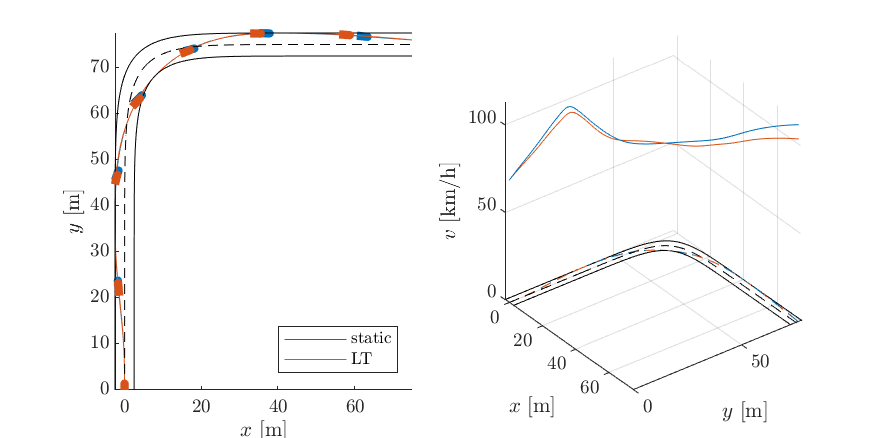
\includegraphics{figures/pep2_comp_posplot.pdf}
    \caption{Time-optimal right-hand turn maneuver for ST model with and without load transfer. The rectangles indicate the position and direction of the vehicle each second.}
    \label{fig:pep2_comp_posplot}
\end{figure}

\begin{figure}[h!]
    \centering
    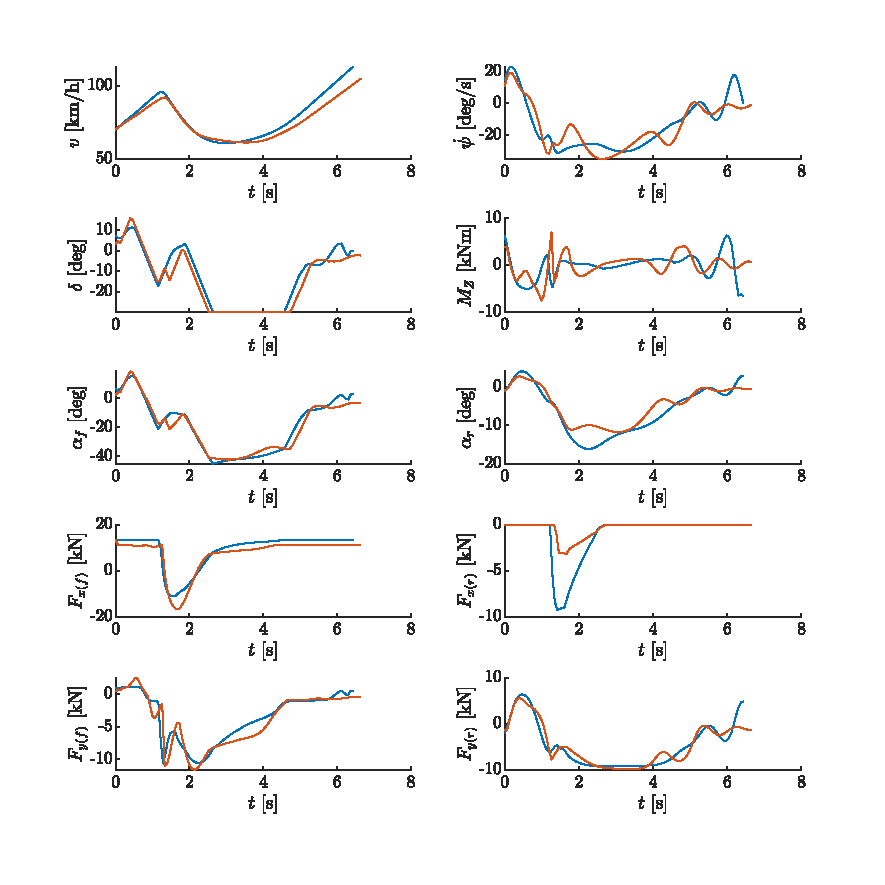
\includegraphics{figures/pep2_comp_detailplot.pdf}
    \caption{Variables of the vehicle model during the time-optimal right-hand turn maneuver with and without load transfer.}
    \label{fig:pep2_comp_detailplot}
\end{figure}

\subsection{Vopt vs. Topt}
As presented in the previous section, the output velocity optimized solution results in the pendulum turn Figures-\ref{fig:pep2_TVcomp_posplot} and \ref{fig:pep2_TVcomp_detailedplot} show the time optimal (topt) and velocity optimized (vopt) solutions for the right-hand turn maneuver for the ST-model with LT. 

\begin{figure}[h!]
    \centering
    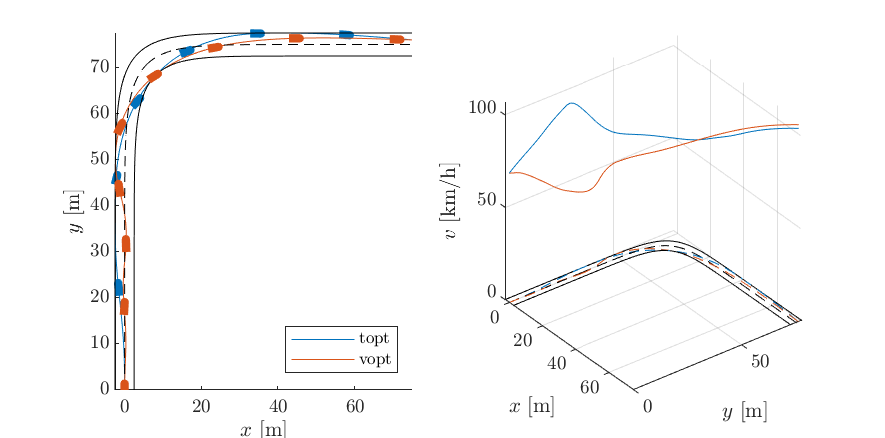
\includegraphics{figures/pep2_TVcomp_posplot.pdf}
    \caption{Trajectory in the XY-plane for time and velocity optimized right-hand turn maneuver. The rectangles indicate the position and direction of the vehicle each second.}
    \label{fig:pep2_TVcomp_posplot}
\end{figure}

\begin{figure}[h!]
    \centering
    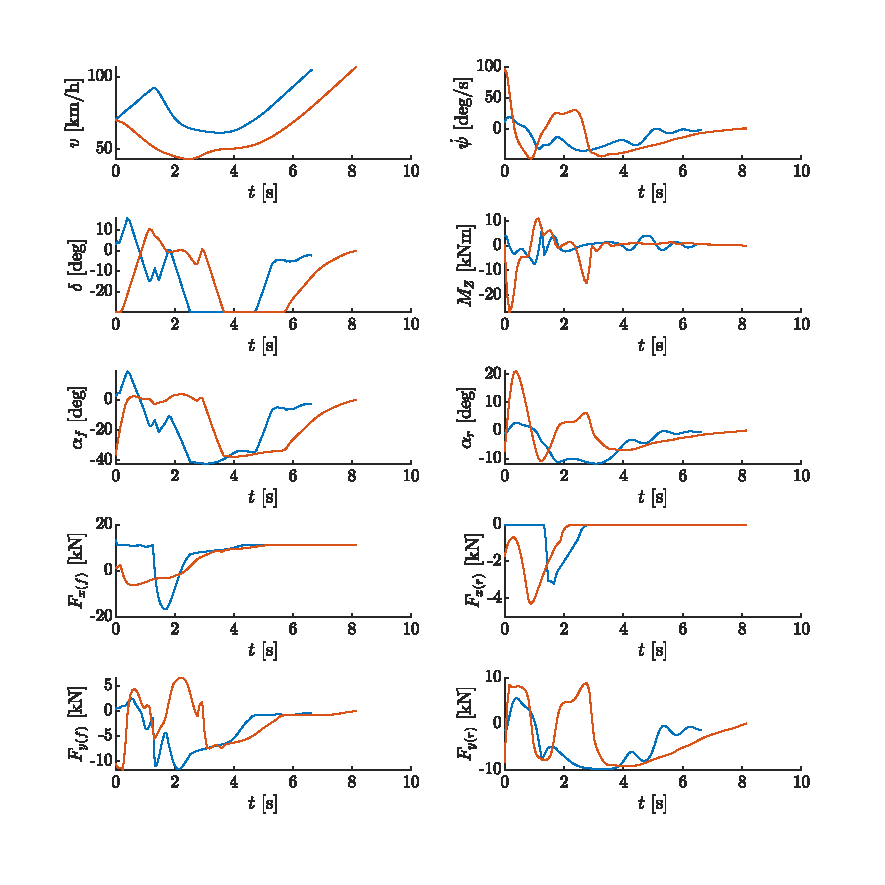
\includegraphics{figures/pep2_TVcomp_detailplot.pdf}
    \caption{Variables of the vehicle model during the time and velocity optimal right-hand turn maneuver.}
    \label{fig:pep2_TVcomp_detailedplot}
\end{figure}

The results of the final time and speed for the time and velocity optimal problem (Min $t$, and Max $v_f$) at the end of the maneuver are summarized in Table~\ref{tab:opt_res_num_pep2_TV}. 
From the table, it is clear that at $Y_o = 0$, Case-V (pendulum turn case) is about 1.5\,m/s faster but takes about 1\,s more to complete the maneuver. 
\begin{table}[h!]
    \centering
    \begin{tabular}{c|c|c|c}
        & & $t_f$ & $v_f$\\
        \hline
        \textbf{topt} & Min $t_f$ & 6.64\,s & 29.1 m/s (104.77\,km/h)\\
        \textbf{vopt} & Max $v_f$ & 8.15\,s & 29.66 m/s (106.78\,km/h)\\
    \end{tabular}
    \caption{Time and speed for the ST-model with LT for the two optimization cases topt and vopt the end of the maneuver, $Y_o = 0$.}
    \label{tab:opt_res_num_pep2_TV}
\end{table}

\clearpage
\subsection{Effect of road friction}
The road friction is changed to wet asphalt and snow conditions, the results are shown in Figures~\ref{fig:pep2_FricComp_posplot} and~\ref{fig:pep2_FricComp_posplot} From the figures, it is clear that the time and velocity optimized trajectories and velocity profiles are closer than for the case with dry and wet asphalt. 

\begin{figure}[h!]
    \centering
    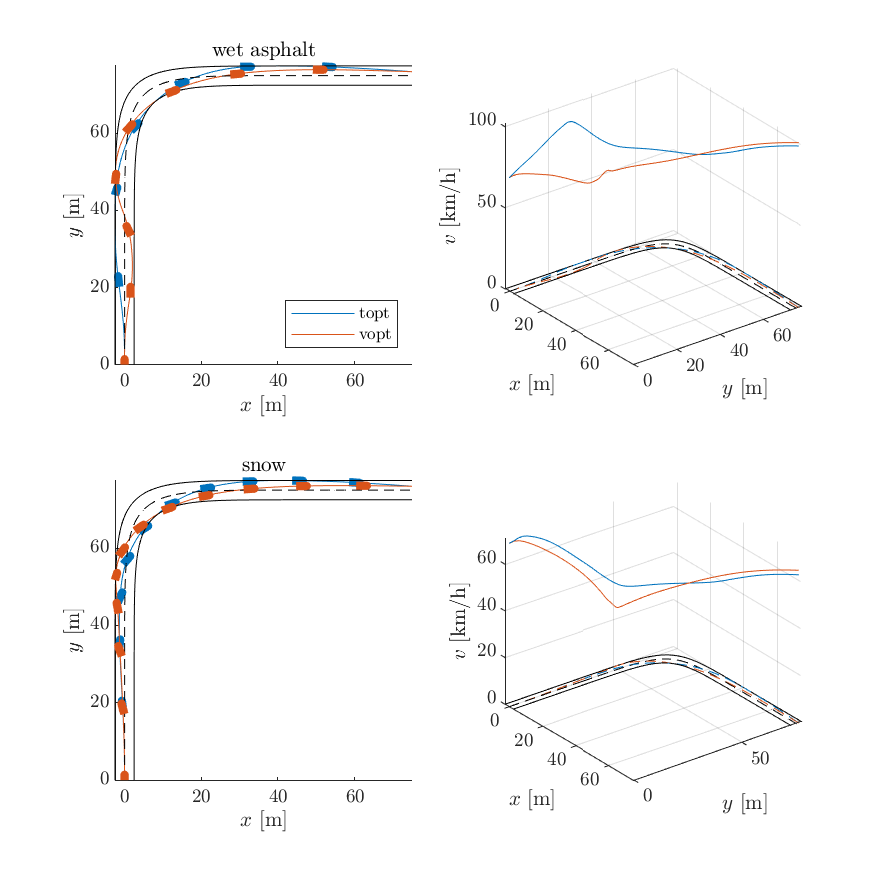
\includegraphics{figures/pep2_FricComp_posplot.pdf}
    \caption{Trajectory in the XY-plane for time and velocity optimized right-hand turn maneuver for wet ahsplat and snow conditions. The rectangles indicate the position and direction of the vehicle each second.}
    \label{fig:pep2_FricComp_posplot}
\end{figure}

\begin{figure}[h!]
    \centering
    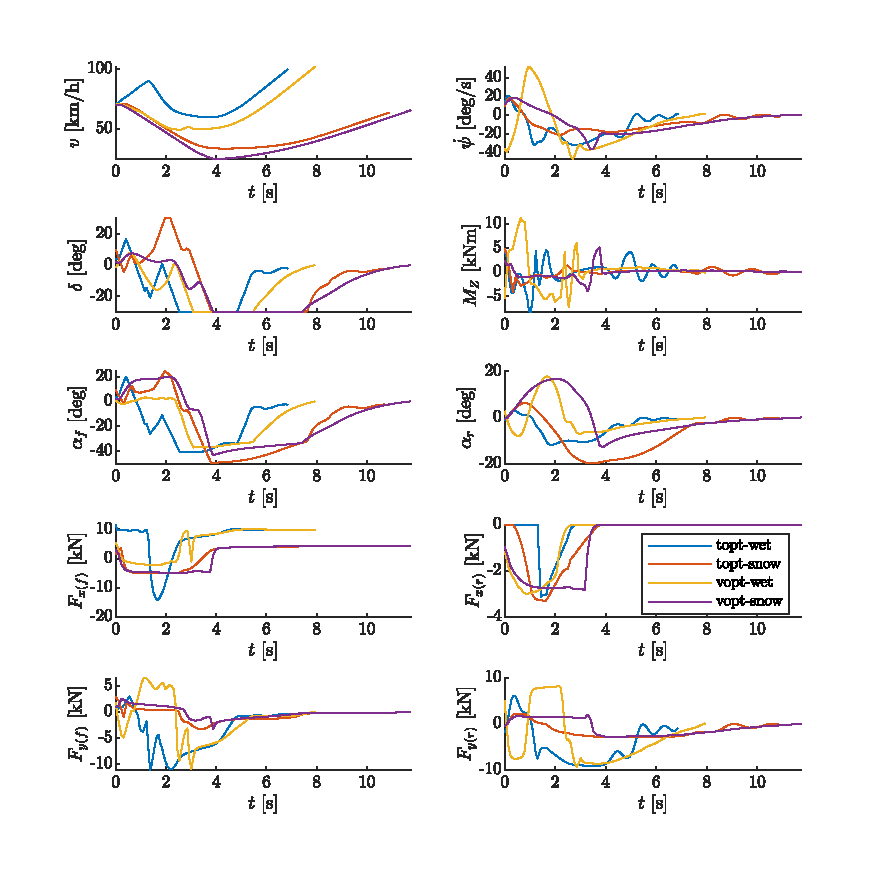
\includegraphics{figures/pep2_FricComp_detailplot.pdf}
    \caption{Variables of the vehicle model during the time and velocity optimal right-hand turn maneuver for wet asphalt and snow conditions.}
    \label{fig:pep2_FricComp_detailplot}
\end{figure}

\clearpage
The results of the final time and speed for the time and velocity optimal problem (Min $t$, and Max $v_f$) at the end of the maneuver for different road conditions are summarized in Table~\ref{tab:opt_res_num_pep2_fric}. 

\begin{table}[h!]
    \centering
    \begin{tabular}{c|c|c|c|c|c|c|c}
        & & \multicolumn{2}{c|}{Dry Asphalt} & \multicolumn{2}{c|}{Wet Asphalt} & \multicolumn{2}{c}{Snow}\\
        & & $t_f$ & $v_f$ & $t_f$ & $v_f$ & $t_f$ & $v_f$\\
        \hline
        \textbf{topt} & Min $t_f$ & 6.64\,s & 29.1 m/s & 6.86\,s & 27.68\,m/s & 10.9\,s & 17.64\,m/s\\
        & & & 104.77\,km/h & & 99.65\,km/h & & 63.49\,km/h\\
        \textbf{vopt} & Max $v_f$ & 8.15\,s & 29.66 m/s & 7.94\,s & 28.23\,m/s & 11.77\,s & 18.18\,m/s\\
        & & & 106.78\,km/h & & 101.69\,km/h & & 65.43\,km/h\\
    \end{tabular}
    \caption{Time and speed for the ST-model with LT for time and velocity optimized scenarios at the end of the maneuver, $Y_o = 0$, with different road frictions.}
    \label{tab:opt_res_num_pep2_fric}
\end{table}

From Figure~\ref{fig:pep2_FricComp_detailplot} it is clear that at no point in time is the velocity of the vehicle for vopt greater than topt but they do get close during snow conditions. This implies that the pendulum turn is not 'viable', even if there is a long straight after the maneuver. However, with a 9-DoF model with load transfer, one can perhaps observe the difference in acceleration of the pendulum turn (vopt) when compared to the time-optimal solution. 

\section*{Code}

The source codes for this problem can be found at \newline \href{https://github.com/arvba41/optimal_vehicle_maneuvers/blob/main/uppgift/pep1}{https://github.com/arvba41/optimal\_vehicle\_maneuvers}.

% \subsection{Effect of change in inertia}
% The mass and the inertia of the vehicle are increased by 12\,\%, and the results are shown in Figures~\ref{fig:pep2_FricComp_posplot} and~\ref{fig:pep2_FricComp_posplot} From the figures, it is clear that the time and velocity optimized trajectories and velocity profiles are closer than for the case with dry and wet asphalt. 


% \pagebreak
% The width of a column is:
% \printinunitsof{mm}\prntlen{\textwidth} (\printinunitsof{in}\prntlen{\textwidth}) \\
% The height of a column is:
% \printinunitsof{mm}\prntlen{\textheight} (\printinunitsof{in}\prntlen{\textheight}) \\



\end{document}